\documentclass[12pt]{article}

%%%%%%%%%%%%%%%%%%%%%%%%%%
%%%  COMMON PACKAGES  %%%%
%%%%%%%%%%%%%%%%%%%%%%%%%%

\usepackage{amsmath}
\usepackage{amssymb}
\usepackage{amsfonts}
\usepackage{graphicx}
\usepackage[utf8]{inputenc}
\usepackage{amsthm}

%%%%%%%%%%%%%%%%%%%%%%%%%%%%%%%%%
%%%  UNUSUAL PACKAGES        %%%%
%%%  Uncomment as necessary. %%%%
%%%%%%%%%%%%%%%%%%%%%%%%%%%%%%%%%

%% MATH AND PHYSICS SYMBOLS
%% ------------------------
\usepackage{slashed}       % \slashed{k}
\usepackage{mathrsfs}      % Weinberg-esque letters
\usepackage{pifont}        % check marks
\usepackage{bbm}           % \mathbbm{1} 
%\usepackage[normalem]{ulem} % for \sout
\usepackage{cancel}


%% CONTENT FORMAT AND DESIGN
%% -------------------------
\usepackage[dvipsnames]{xcolor}
\usepackage{fancyhdr}		% to put preprint number
\usepackage{lipsum}         % block of text 
\usepackage{framed}         % boxed remarks
\usepackage{subcaption}     % subfigures
\usepackage{cite}           % group cites
%\usepackage{tocloft}       % Table of Contents	
\usepackage{xspace}			% spacing after macros
\usepackage{listings}       % code environment	
\lstset{
		basicstyle=\ttfamily\footnotesize,
		breaklines=true,
		backgroundcolor=\color{gray!15!white}}


%% TABLES IN LaTeX
%% ---------------
\usepackage{booktabs}      % professional tables
\usepackage{nicefrac}      % fractions in tables,
\usepackage{multirow}      % multirow elements 
\usepackage{arydshln} 	    % dashed lines in arrays

%% Other Packages and Notes
%% ------------------------
\usepackage[font=small]{caption} % small capt font
\usepackage{float}         % for strict placement e.g. [H]


%% CUSTOM PACKAGES
%% ---------------
\usepackage{tikzfeynman}   % Flip's rules Feynman Diagrams



%%%%%%%%%%%%%%%%%%%%%%%%%%%%%%
%%%  DOCUMENT PROPERTIES  %%%%
%%%%%%%%%%%%%%%%%%%%%%%%%%%%%%
\usepackage[margin=2cm]{geometry}   % margins
\graphicspath{{figures/}}			% figure folder
\numberwithin{equation}{section}    % set equation numbering


%% References in two columns, smaller
%% http://tex.stackexchange.com/questions/20758/bibliography-in-two-columns-section-title-in-one
\usepackage{multicol}
\usepackage{etoolbox}
\usepackage{relsize}
\patchcmd{\thebibliography}
  {\list}
  {\begin{multicols}{2}\smaller\list}
  {}
  {}
\appto{\endthebibliography}{\end{multicols}}


% Change list spacing
% from: http://en.wikibooks.org/wiki/LaTeX/List_Structures#Line_spacing
\let\oldenumerate\enumerate
\renewcommand{\enumerate}{
  \oldenumerate
  \setlength{\itemsep}{1pt}
  \setlength{\parskip}{0pt}
  \setlength{\parsep}{0pt}
}

\let\olditemize\itemize
\renewcommand{\itemize}{
  \olditemize
  \setlength{\itemsep}{1pt}
  \setlength{\parskip}{0pt}
  \setlength{\parsep}{0pt}
}


%%%%%%%%%%%%%%%%%%%%%%%%%%%
%%%  (RE)NEW COMMANDS  %%%%
%%%%%%%%%%%%%%%%%%%%%%%%%%%

%% FOR `NOT SHOUTING' CAPS (e.g. acronyms)
%% ---------------------------------------
\newcommand{\acro}[1]{\textsc{\MakeLowercase{#1}}}    

%% COMMON PHYSICS MACROS
%% ---------------------
\renewcommand{\tilde}{\widetilde}   % tilde over characters
\renewcommand{\vec}[1]{\mathbf{#1}} % vectors are boldface
\newcommand{\dbar}{d\mkern-6mu\mathchar'26}    % for d/2pi
\newcommand{\ket}[1]{\left|#1\right\rangle}    % <#1|
\newcommand{\bra}[1]{\left\langle#1\right|}    % |#1>
\newcommand{\Xmark}{\text{\sffamily X}}        % cross out

%% COMMANDS FOR TEMPORARY COMMENTS
%% -------------------------------
\newcommand{\comment}[2]{\textcolor{red}{[\textbf{#1} #2]}}
\newcommand{\flip}[1]{{
	\color{green!50!black} \footnotesize [\textbf{\textsf{Flip}}: \textsf{#1}]
	}}


%% COMMANDS FOR TOP-MATTER
%% -----------------------
\newcommand{\email}[1]{\href{mailto:#1}{#1}}
\newenvironment{institutions}[1][2em]{\begin{list}{}{\setlength\leftmargin{#1}\setlength\rightmargin{#1}}\item[]}{\end{list}}


%% COMMANDS FOR LATEXDIFF
%% ----------------------
%% see http://bit.ly/1M74uwc
\providecommand{\DIFadd}[1]{{\protect\color{blue}#1}} %DIF PREAMBLE
\providecommand{\DIFdel}[1]{{\protect\color{red}\protect\scriptsize{#1}}}

%% REMARK: use latexdiff option --allow-spaces
%% for \frac, ref: http://bit.ly/1iFlujR


%%%%%%%%%%%%%%%%%%%%%%%%%%%%%%%%%%%%%%%%%%%%%%
%%%  TIKZ COMMANDS FOR EXTERNAL DIAGRAMS  %%%%
%%%  requires -shell-escape               %%%%
%%%  in texpad 1.7: prefs > shell esc sec %%%%
%%%%%%%%%%%%%%%%%%%%%%%%%%%%%%%%%%%%%%%%%%%%%%

%% For exporting tikz figures as into a ./tikz/ subfolder.
%% It is useful if you want pdf versions of the tikz diagrams or
%% if you need to speed up compilation of a large document with
%% many tikz diagrams.

%\write18{} % Careful with this!
%\usetikzlibrary{external}
%\tikzexternalize[prefix=tikz/] % folder for external pdfs


%%%%%%%%%%%%%%%%%%%
%%%  HYPERREF  %%%%
%%%%%%%%%%%%%%%%%%%

%% This package has to be at the end; can lead to conflicts

\usepackage[
	colorlinks=true,
	citecolor=green!50!black,
	linkcolor=NavyBlue!75!black,
	urlcolor=green!50!black,
	hypertexnames=false]{hyperref}


%%%%%%%%%%%%%%%%%%%%%
%%%  TITLE DATA  %%%%
%%%%%%%%%%%%%%%%%%%%%

%% PREPRINT NUMBER USING fancyhdr
%% Don't forget to set \thispagestyle{firststyle}
%% ----------------------------------------------
\renewcommand{\headrulewidth}{0pt} 	% no separator
\setlength{\headheight}{15pt} 		% min to avoid fancyhdr warning
\fancypagestyle{firststyle}{
	\rhead{\footnotesize%
%	\texttt{UCI-TR-2016-XX}\\ %% Uncomment for additional preprint #s
	\texttt{UCR-PHYS-165-W2018-A}%
	}}

%% TOC overwrites fancyhdr, here's a fix
%% http://tex.stackexchange.com/questions/167828/difficult-with-fancyhdr-and-table-of-contents
\usepackage{etoc}
\renewcommand{\etocaftertitlehook}{\pagestyle{plain}}
\renewcommand{\etocaftertochook}{\thispagestyle{firststyle}}



\begin{document}

%\thispagestyle{empty}		% default if no preprint #
\thispagestyle{firststyle} 	% to include preprint

\begin{center}

    {\huge \bf P165: Introduction to Particle Physics}

    \vskip .7cm

%% SINGLE AUTHOR FORMAT
%% --------------------
	Prof.~\textbf{Flip Tanedo} %\\
	(\texttt{\footnotesize \email{flip.tanedo@ucr.edu}})

	\vspace{-1em}
    \begin{institutions}[2.25cm]
    \footnotesize
    {\it 
	    Department of Physics \& Astronomy, 
	    University of  California, Riverside, 
	    {CA} 92521	    
	    }    
    \end{institutions}


\end{center}




%%%%%%%%%%%%%%%%%%%%%
%%%  ABSTRACT    %%%%
%%%%%%%%%%%%%%%%%%%%%

\begin{abstract}
\noindent 
These are course notes for Physics 165.
\\
\textbf{These notes are in progress}. Last update: \today
\end{abstract}



\small
\setcounter{tocdepth}{2}
\tableofcontents
\normalsize
%\clearpage


%%%%%%%%%%%%%%%%%%%%%
%%%  THE MEAT    %%%%
%%%%%%%%%%%%%%%%%%%%%

%% Use \input if you have separate files.
%% \include is `smarter' (creates separate aux files
%% for each tex file) and hence more efficient, 
%% but it automatically puts a page break
%% between included files. Input doesn't do this.

\section{Preliminaries}

\subsection{Units}
% Lecture 1

We work in \textbf{natural units}\footnote{For a very nice reference, see Jaffe's \acro{MIT} Quantum Theory Notes: Natural Units, \url{https://stuff.mit.edu/afs/athena/course/8/8.06/spring08/handouts/units.pdf}}. This means that we will measure everything in units of electron volts, usually MeV or GeV. The rule for natural units is:
\begin{align}
	\hbar = c = 1 \ .
\end{align}
How can this be? If you open up the \acro{PDG} particle booklet (``the \acro{PDG}'') to their table of constants, you'll find that
\begin{align}
	c & = 3 \times 10^8~\text{m}/\text{s}
	\\
	\hbar &= 7 \times 10^{-22}~\text{MeV~s} \ .
\end{align}
This means that if $c=1$, we can write
\begin{align}
	\text{second} = 3\times 10^8 \, \text{meter} \ ,
\end{align}
which is precisely what we mean by a \emph{light second}: the distance something would travel if it were traveling at the speed of light. 

Why is this useful? If you're driving from Riverside to Irvine at rush hour, you'd be happy to hit 20 mph. Why don't we define ``natural on the highway 91'' units where $c_\text{hwy 91} = 20~\text{mph}$ is used.

For example: Han Solo claims to have done the Kessel Run in 12 parsecs. For most Star Wars fans, this doesn't make any sense: a parsec is a unit of distance, and Solo used it in place of a unit time. However, the relation $c=1$ gives us a way to show how to convert one type of unit to another. The trick is to just multiply by one in a useful way:
\begin{align}
	12\,\text{pc}
	= 12 \times 3 \times 10^{16}\,\text{m}\times (1/c)
%	\\
	= 4\times 10^{17}\, \text{m}
	\times\left(\frac{1}{3\times 10^{8}\,\text{m}/\text{s}}\right)
%	\\
	= 10^9\, \text{s} \ .
\end{align}
How did we know that 1~pc$= 3\times 10^{18}~$m? We looked it up in the \acro{PDG}. By the way, $10^9$ seconds is not particularly impressive---that's 30 years!

Similarly, the relation $\hbar = 1$ lets us convert between energy and time. The Large Hadron Collider smashes together protons at an energy of about 10 TeV. This corresponds to an inverse time, which by $c=1$ we can convert into an inverse length scale. We can find the value of this length scale in meters by ``multiplying by one'' to convert unis:
\begin{align}
	10~\text{TeV} \times
	\left(\frac{1}{7\times 10^{22}\,\text{MeV}\,\text{s}}\right)
	\times\left(\frac{1}{3\times 10^{8}\,\text{m}/\text{s}}\right)
	= 
	\frac{1}{10^{-20}\,\text{m}} \ .
\end{align}
The size of an atom is about an Angstrom, which is $10^{-10}~$m. From this we may guess that the \acro{LHC} probes length scales $10^{10}$ times smaller than an atom. This turns out to be too na\"ive---we'll see why in this class---but the principle is clear: high-energy colliders are \emph{microscopes}. The higher the energy, the smaller the length scale being probed. This is why particle physics is also known as \textbf{high-energy physics}. 

\subsection{Kinematics}
% Lecture 1

\textbf{Kinematics} has to do with how we describe motion. Since we're going to high energies, it is important to include the effects of special relativity. You should be familiar with four-vectors and Lorentz transformations---we will be using them later in these lectures. For now, however, we're going to limit ourselves to three useful rules:
\begin{enumerate}
	\item Energy is conserved in any process.
	\item Momentum is conserved in any process.
	\item The Einstein relation,
\begin{align}
	E^2 = m^2 + \vec{p}^2 \ .
\end{align}
\end{enumerate}
%
Recall that the first two rules come from the invariance of special relativity with respect to time translations and space translations, respectively. We will assume these features in this course, but it may be worth remembering that our universe is decidedly not time-translation invariant: this is why photons from the cosmic microwave background are \emph{red-shifted}: they lose energy as the universe expands.

The Einstein relation is the relativistic version of the famous $E=mc^2$. Those with a mathematical inclination may want to read this as
\begin{align}
	m^2 = E^2 - \vec{p}^2 \ ,
\end{align}
which is nice because it describes an invariant (mass) in terms of the Lorentz norm of the momentum four-vector, $p^2 = E^2-\vec p^2$ where $p_\mu = (E, \vec p)$. By the way, by writing this we have chosen the `mostly-minus' metric. This is a convenient choice because it means that squared particle masses are positive. We'll dig more deeply into four-vectors as we progress. 

It is useful to introduce some nomenclature. A particle whose energy and momenta satisfies the Einstein relation is said to be \textbf{on-shell}. In contrast, a particle that is \emph{not} on-shell is called \textbf{virtual}. This should sound strange! We just said that the Einstein relation is a rule---why should we separate particles into those that do and do not obey the rule? The answer is that particle physics is a quantum theory, and not all quantum particles are on-shell.

\section{Quantum Mechanics}

Particle physics is inherently quantum. If you want to study a subatomic particle, you do not simply pick it up and look at it. 
%
There are remarkably few particles that we can actually detect directly. Most particles only exist in a fleeting moment in a quantum mechanical sense. Was it there? Was it not? It Schr\"odinger's cat dead or alive in between observations?

The lesson of quantum mechanics is that we can only say definite things about observed states. This is the classic two-slit experiment. If you detect a particle on the other side of the double-slit, did it pass through the first slit or the second? Quantum mechanically, it took \emph{both} paths. Similarly, if you started with some particle configuration $\left|\text{in}\right\rangle$ and ended up with some other configuration $\left|\text{out}\right\rangle$, then all we can do is ask about
\begin{align}
	\langle \text{out} | (\text{time evolution}) | \text{in}\rangle \ ,
\end{align}
where ``(time evolution)'' refers to the time evolution operator. This operator encodes the \textbf{dynamics} of a theory and tells us about all possible allowed histories between the initial and final states. For now what is important to note is that everything that happens ``in between'' the initial and final states has to be summed over. In the same way that the interference pattern in the double slit experiment comes from summing the amplitudes of different paths, the amplitude $\langle \text{out} | (\text{time evolution}) | \text{in}\rangle $ involves a sum over all possible dynamics that aren't directly observed. 


The punchline is that in this course, we will be focused on two kinds of quantum processes:
\begin{itemize}
	\item \textbf{Scattering}: a two or more particles go to a configuration of two or more particles.
	\item \textbf{Decays}: a single particle turns into two or more particles.
\end{itemize}
To simplify nomenclature, we will use \textbf{scattering} to refer to either type of process.


\subsection{Particle Physics}

A \textbf{model} is a theory of particle physics. We use this nomenclature for two reasons:
\begin{enumerate}
	\item It is a reminder that this is a human construction meant to approximate nature.
	\item It frees up the word `theory' for things like the ``theory of special relativity'' and ``quantum field theory,'' which are the mathematical super-structures that contain our models\footnote{All of our models are quantum field theories; quantum field theory is a general framework to describe models consistently.}.
\end{enumerate}
This isn't ``official'' in any way; I just made it up. Anyway, these are just words. 

For now let us define a \textbf{model} as being composed of two things:
\begin{enumerate}
	\item A list of particles.
	\item A list of interactions between particles. 
\end{enumerate}
In time we will refine these ideas. After all, we haven't said anything about fundamental forces or symmetries. For now, it is much more interesting to just dive right in and see what a model of particle physics looks like.

\section{Quantum electrodynamics}

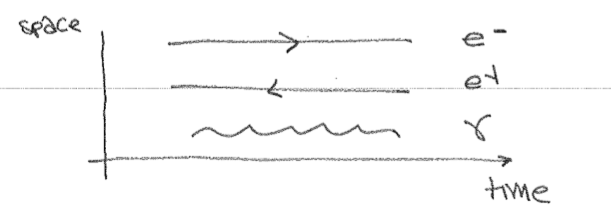
\includegraphics[width=\textwidth]{Lec1_forward}

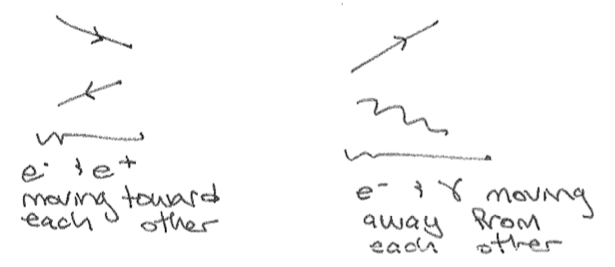
\includegraphics[width=.6\textwidth]{Lec1_noaxis}


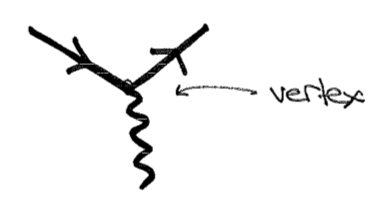
\includegraphics[width=.3\textwidth]{Lec1_vertex}

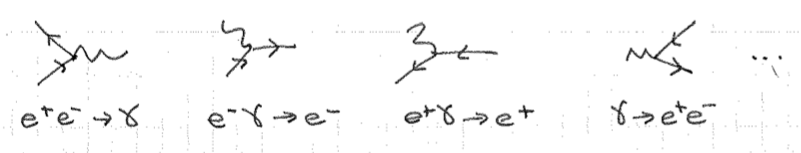
\includegraphics[width=\textwidth]{Lec1_3pt}

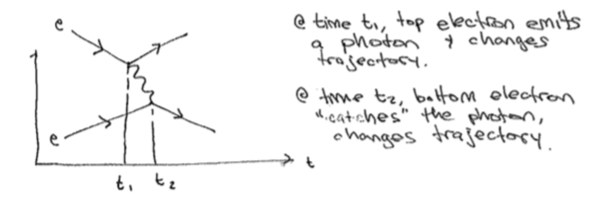
\includegraphics[width=\textwidth]{Lec1_order}


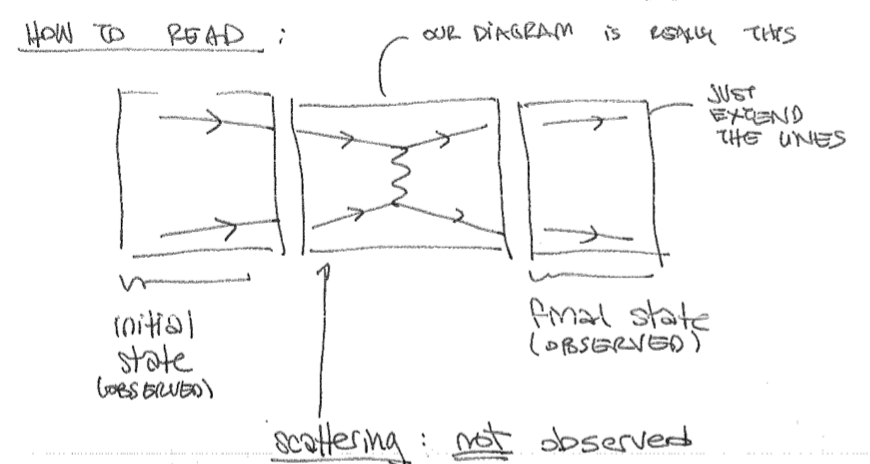
\includegraphics[width=\textwidth]{Lec1_diagram}

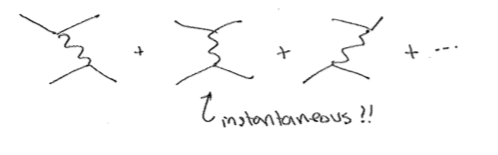
\includegraphics[width=\textwidth]{Lec1_sum}





\section{Particle Botany}

\begin{quote}
\emph{If I could remember the names of these particles, I would have been a botanist.}\\
	-- Enrico Fermi	(via Leon Lederman\footnote{\url{https://quoteinvestigator.com/2017/07/19/particles/}})
\end{quote}



\section*{Acknowledgements}


%
\textsc{p.t.}\ thanks 
\emph{your name here}
for useful comments and discussions. 
%
\textsc{p.t.} thanks the Aspen Center for Physics (NSF grant \#1066293) for its hospitality during a period where part of this work was completed.

%% Appendices
% \appendix


%% Bibliography
\bibliographystyle{utphys} 	% arXiv hyperlinks
% \bibliography{bib title without .bib}


\end{document}